\section{Modelli di formazione globali. Costruzione popolazioni sintetiche}

\begin{frame}{Modelli di formazione globali}
\begin{figure}[!ht]
	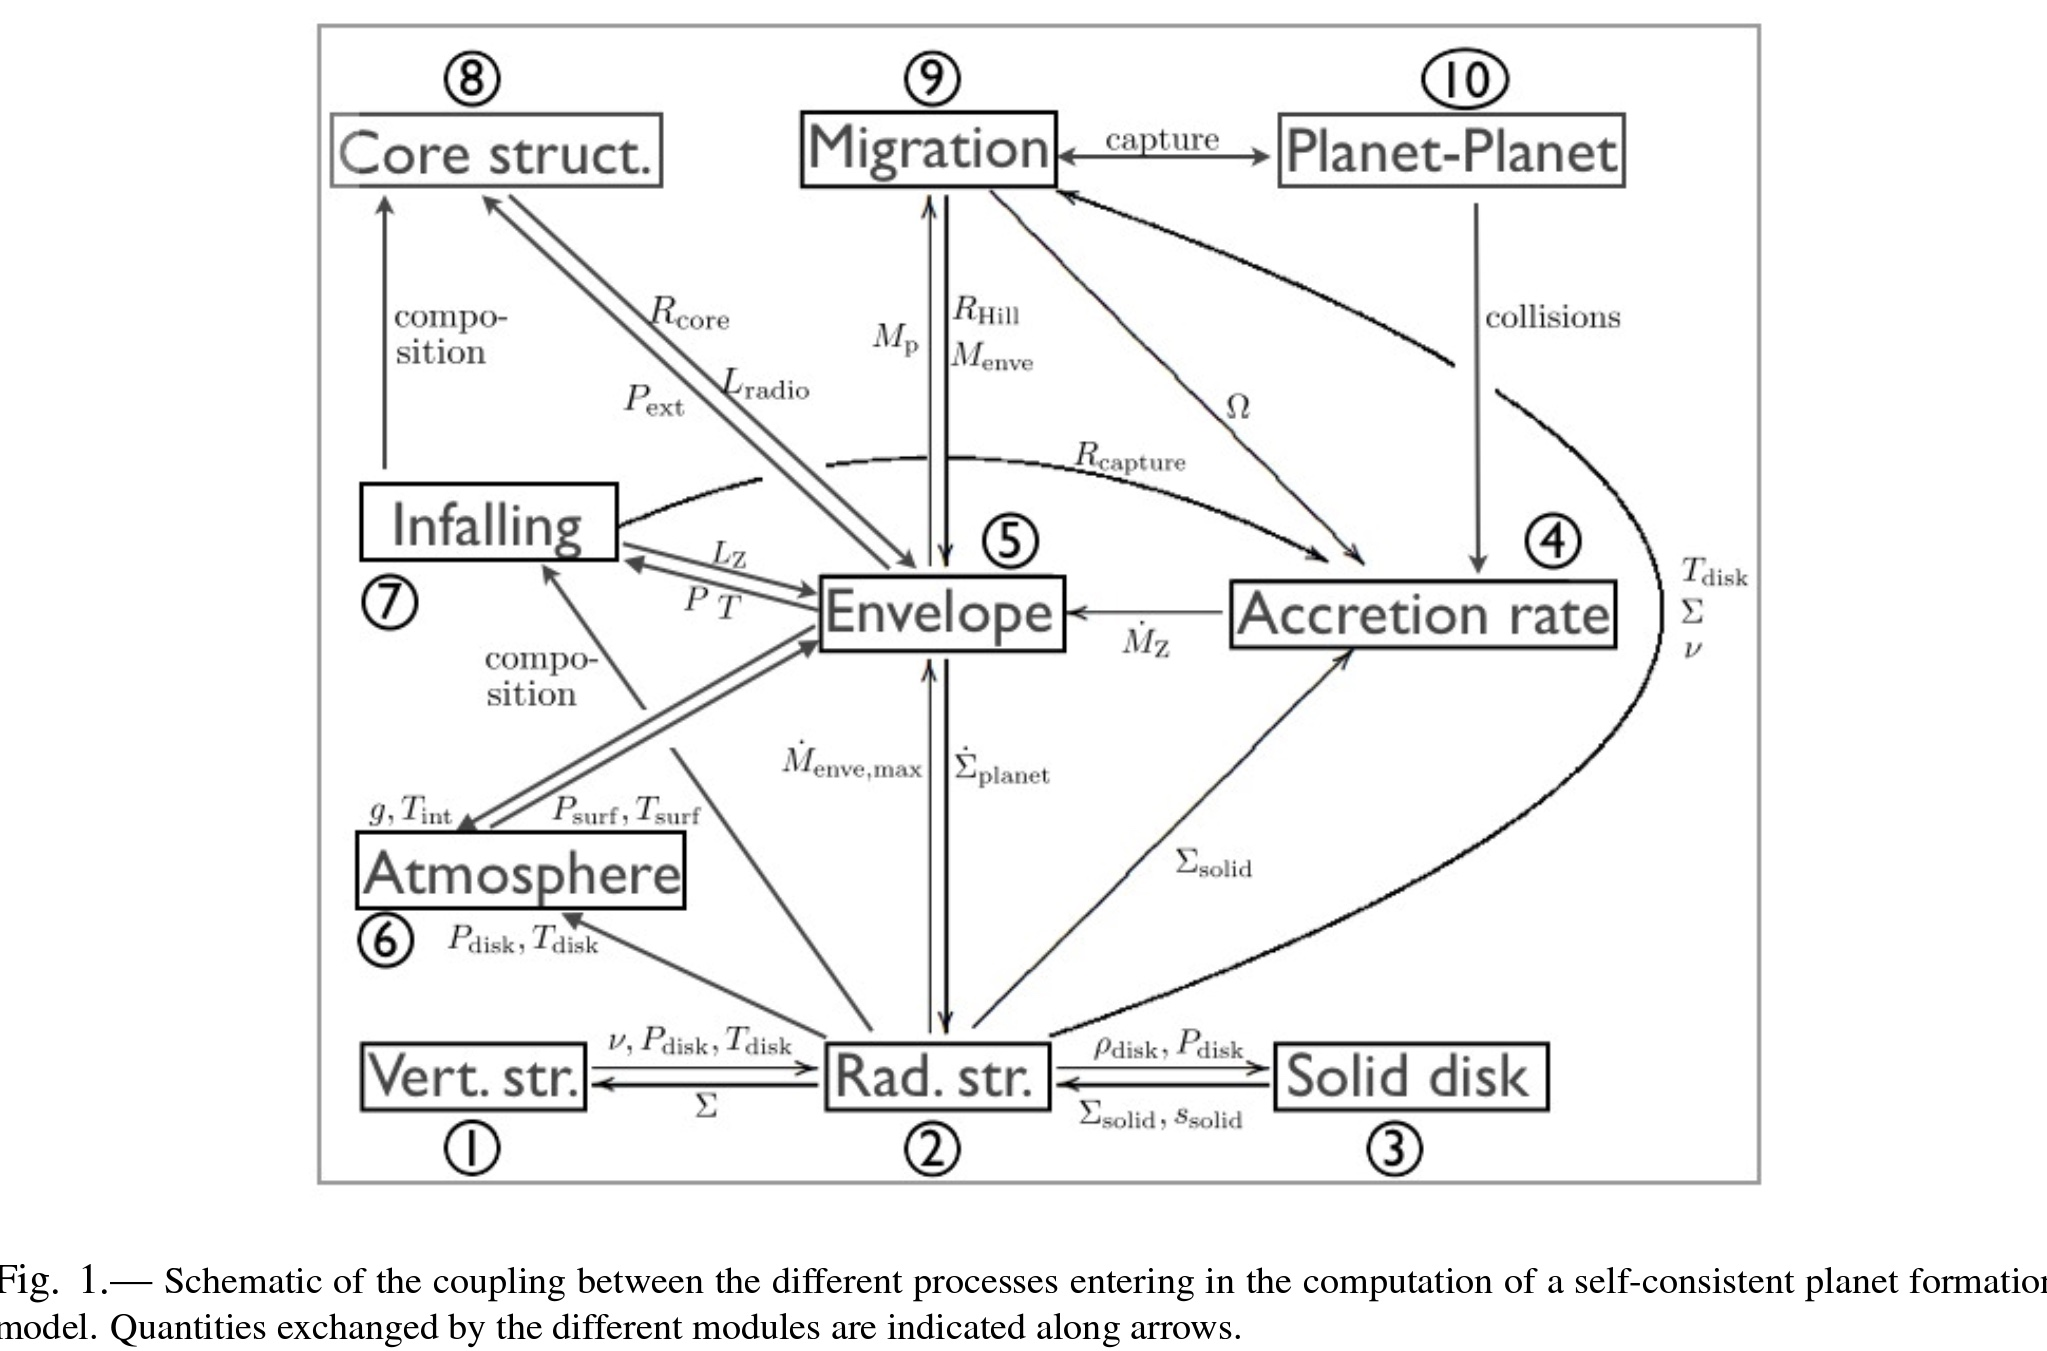
\includegraphics[trim={8cm 5cm 8cm 0},clip, keepaspectratio, width=0.7\textwidth]{GFM}
	\caption{Da \cite{benz2014planet}.}\label{fig:GFM}
\end{figure}
\end{frame}

\begin{wordonframe}{GFM}
contenu...
\end{wordonframe}

\begin{frame}{Distribuzione iniziale caratteristiche dischi protoplanetari}
	\begin{figure}[!ht]
		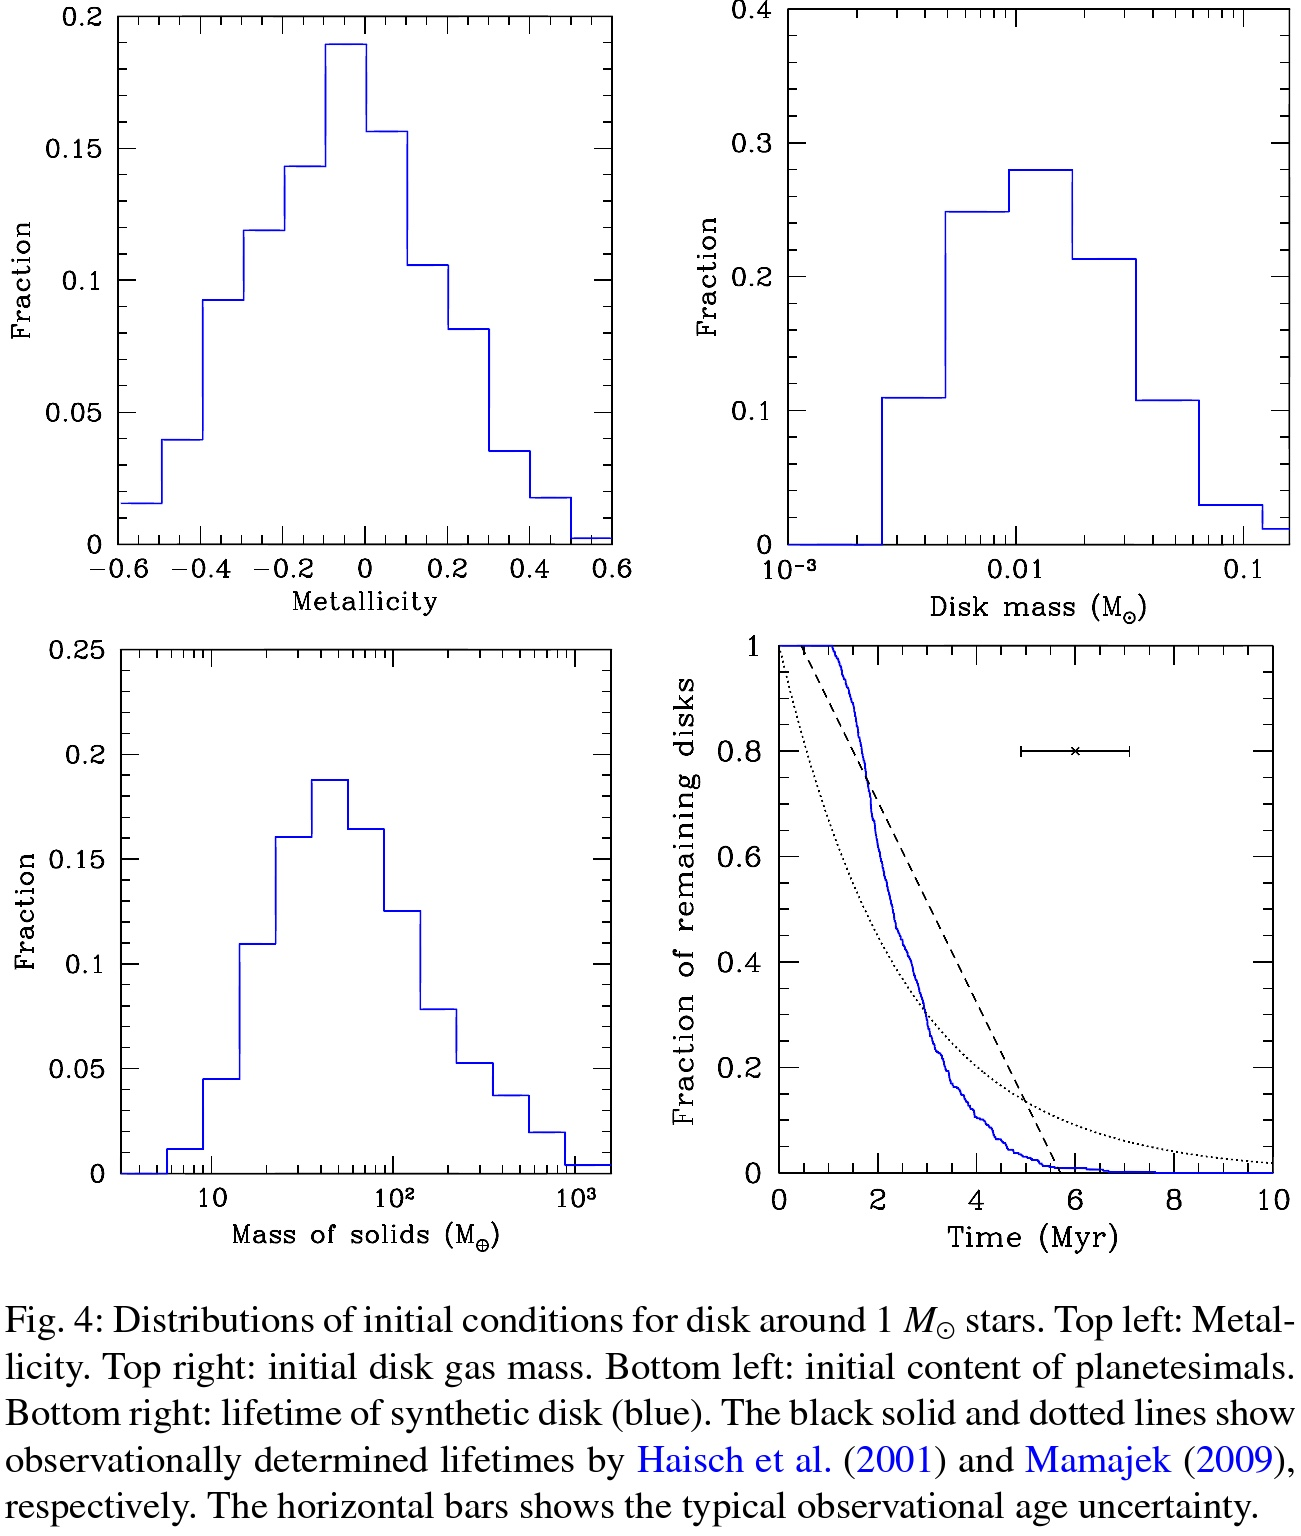
\includegraphics[trim={0cm 10cm 0 0},clip, keepaspectratio,width=0.7\textwidth]{initdistro}
		\caption{Da \cite{mordasini2018planetary}.}\label{fig:initdistro}
	\end{figure}
\end{frame}

\begin{frame}[allowframebreaks]{Condizioni iniziali ed evoluzione del disco protoplanetario}
\begin{block}{Evoluzione disco proto-planetario}
\begin{align*}
&\TDy{t}{\Sigma}=\frac{1}{r}\PDof{r}[3r\expy{1/2}\PDof{r}(\nu\Sigma r\expy{1/2})]+\dot{\Sigma}_w(r)+\dot{\Sigma}_{embryo}(r)\label{eq:diskaccrphev-m18}\\
&\dot{\Sigma}_w(a)=\left\{\begin{array}{c}0\\\frac{\dot{M}_w}{2\pi(a_{max}-R_g)a}\\\end{array}\right.\\
&\Sigma(a,t=0)=\Sigma_0(\frac{r}{1AU})\expy{p_g}\Exp{[-(\frac{r}{R_o})\expy{2+p_g}]}(1-\sqrt{\frac{r}{R_i}})
\end{align*}
\end{block}

\begin{block}{Parametri di montecarlo}
\begin{itemize}
	\item $M_{disk}$: distribuzione gaussiana di $\log{M_{disk}}$ ($\mu_{obs}=0.042\msun{}$, $\sigma_{obs}$)
	\item $\alpha$, $\dot{M}_w$: $t_{disk}(\alpha,\Sigma_0,\dot{M}_w)=\SI{3}{\mega\year}$.
	
	($\dot{M}_w=\SIrange{5e-10}{3e-8}\msun{}/\si{\year}$, $\alpha=\num{7e-3}$)
\end{itemize}
\end{block}

\end{frame}

\begin{wordonframe}{Evoluzione disco protoplanetario e condizioni iniziali}
La distribuzione di massa e la frazione di dischi protoplanetari per ammassi stellari di et\'a diversa \'e mostrata in figura (\ref{fig:initdistro}). La massa \'e determinata misurando il flusso di emissione termica della polvere: la distribuzione di $\log{M_{disk}}$  \'e gaussiana e per il cluster Ophiuchus la distribuzione \'e fittata da gaussiana con $\mu=-1.38$ ($M_{disk}=0.042\msun{}$) e $\sigma=0.49$.

Il tempo caratteristico del disco \'e determinato dalla viscosit\'a $\alpha$: fissata $\alpha$ compatibile con tempo caratteristico osservato $\tau_{disk}^{obs}\approx\SI{3}{\mega\year}$ e assumendo la distribuzione uniforme nel logaritmo di $\dot{M}_w$, si calcola  $t_{disk}(\alpha,\Sigma_0,\dot{M}_w)$ determinando gli estremi dello fotoevaporazione per riprodurre tempi di vita osservati.

Valori tipici sono $\dot{M}_w=\SIrange{5e-10}{3e-8}\msun{}/\si{\year}$ per $\alpha=\num{7e-3}$.

Nelle popolazione planetaria considerata $\alpha$ \'e fissato sulla base delle osservazioni  ed \'e omogeneo e costante.

\end{wordonframe}

\begin{frame}{Distribuzione iniziale planetesimi ed embrioni planetari}
\begin{block}{Conversione polvere in planetesimi}

	\begin{equation*}
	\Sigma_p(t=0,r)=f_{dg}\eta_{ice}\Sigma_g(t=0,r)
	\end{equation*}
	
	\begin{equation*}
	\frac{f_{D/G}}{f_{D/G\odot}}=10\expy{[\cel{Fe}{}{}{}/\cel{H}{}{}{}]}
	\end{equation*}
	$f_{D/G\odot}\approx\numrange{0.01}{0.02}$ (\cite{lodders2003solar}).
\end{block}
\begin{block}{Posizione iniziale embrioni e tempo di comparsa}
Posizione iniziale: $P(a)\,da\propto d\,\log{a}\propto\const{}$.
Tempo comparsa: accumulo massa planetesimi

\end{block}
\end{frame}

\begin{wordonframe}{Distribuzione iniziale planetesimi/embrioni}
---Distribuzione iniziale planetesimi
Assumendo conversione completa di polvere in planetesimi, la densit\'a superficiale di planetesimi \'e
\begin{equation}
\Sigma_p(t=0,r)=f_{dg}\eta_{ice}\Sigma_g(t=0,r)
\end{equation}
con $f_{dg}$ rapporto gas/polvere (circa metallicit\'a) \'e una parametro casuale con distribuzione che riflette distribuzione di metallicit\'a stellari, $\eta_{ice}$ tiene conto della discontinuit\'a nella distribuzione superficiale di solidi all'iceline.

Sulla scorta della piccola differenza tra composizione solare e composizione meteoritica e assumendo inoltre che il ferro sia un buon indicatore della componente solida  si usa la formula
\begin{equation}
\frac{f_{D/G}}{f_{D/G\odot}}=10\expy{[\cel{Fe}{}{}{}/\cel{H}{}{}{}]}
\end{equation}
con $f_{D/G\odot}\approx\numrange{0.01}{0.02}$ (\cite{lodders2003solar}).
\end{wordonframe}

\section{Caratteristiche popolazioni sintetiche}

\begin{frame}{Popolazione sintetica: traccie di formazione e fase accrescimento gas}

\begin{figure}[!ht]
	\begin{subfigure}[b]{0.48\textwidth}
		\centering
		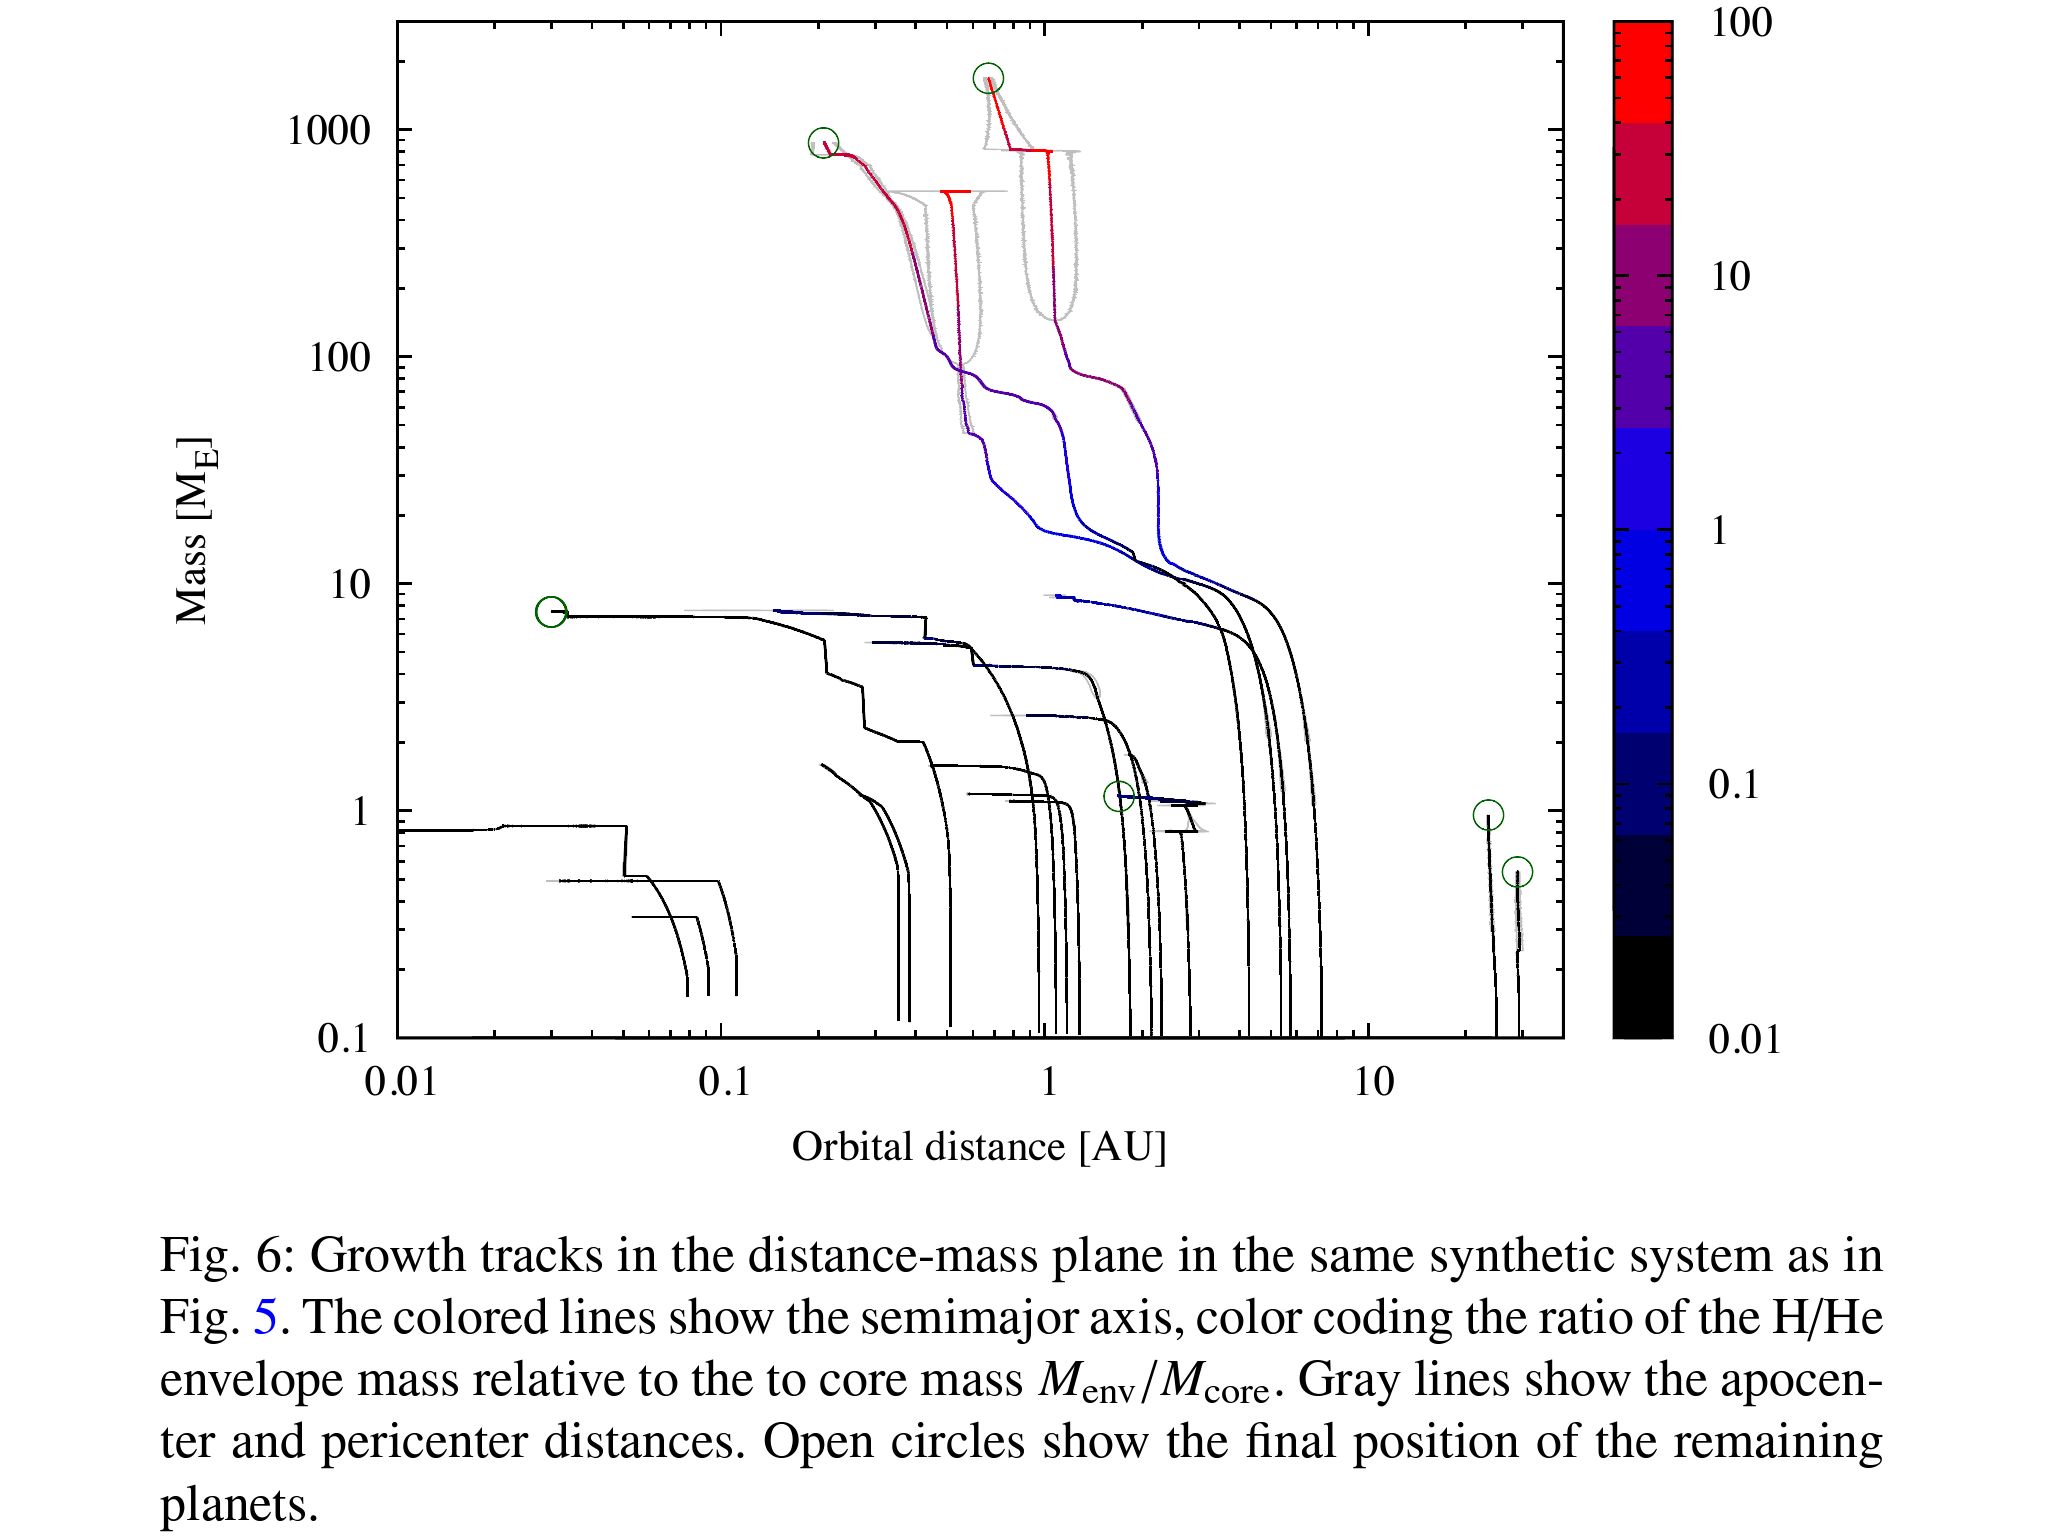
\includegraphics[trim={2cm 12cm 2cm 0},clip, width=0.99\textwidth,keepaspectratio]{track1}
		\caption{Formazione di un sistema planetario nel diagramma $a-M$: alla scomparsa del disco protoplanetario si hanno 2 pianeti giganti, un nettuniano caldo e 3 pianeti terrestri. La scala di colore indica la composizione $\frac{M_e}{M_c}$. Da \cite{mordasini2018planetary}.}\label{fig:track1}
	\end{subfigure}
	~
	\begin{subfigure}[b]{0.49\textwidth}
		\centering
		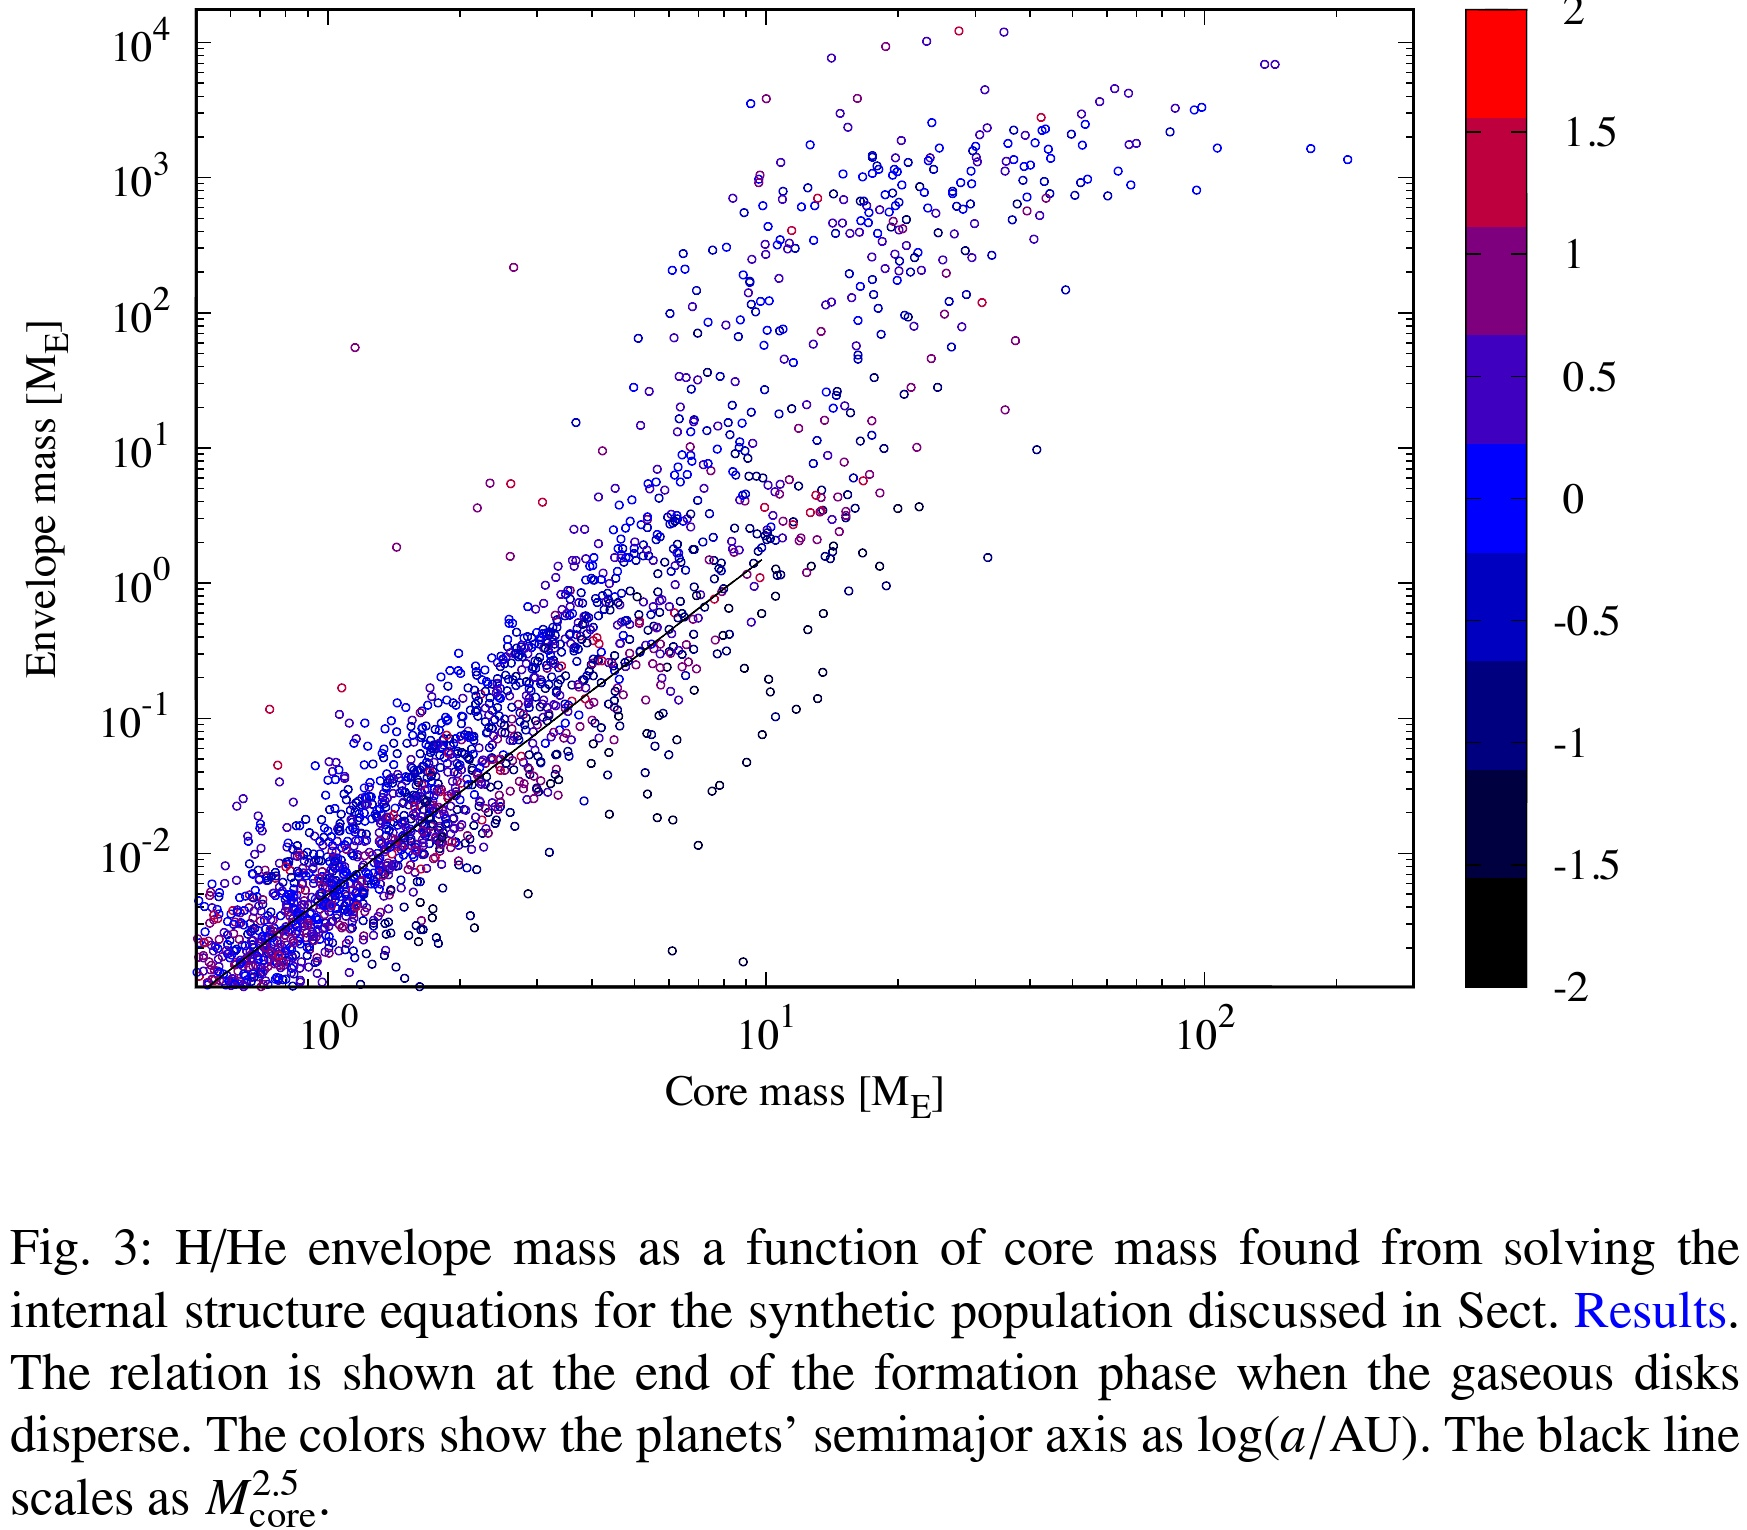
\includegraphics[trim={0cm 12cm 0 0},clip, width=0.99\textwidth,keepaspectratio]{envelopecoresynth}
		\caption{Massa inviluppo gassoso vs massa core. Il colore indica la distanza in $\log{\frac{a}{\si{\astronomicalunit}}}$. La linea continua mostra andamento $M_c\expy{-q_{KH}-1}=M_c\expy{2.5}$ precedente alla fase runaway di accrescimento gassoso. Da \cite{mordasini2018planetary}. }\label{fig:envelopecoresynth}
	\end{subfigure}
\end{figure}
\end{frame}

\begin{wordonframe}{Tracce formazione}
crescendo verso diversity in massa-distanza
\end{wordonframe}

\begin{frame}{Popolazione sintetica nel diagramma massa-distanza}
\begin{figure}[!ht]
	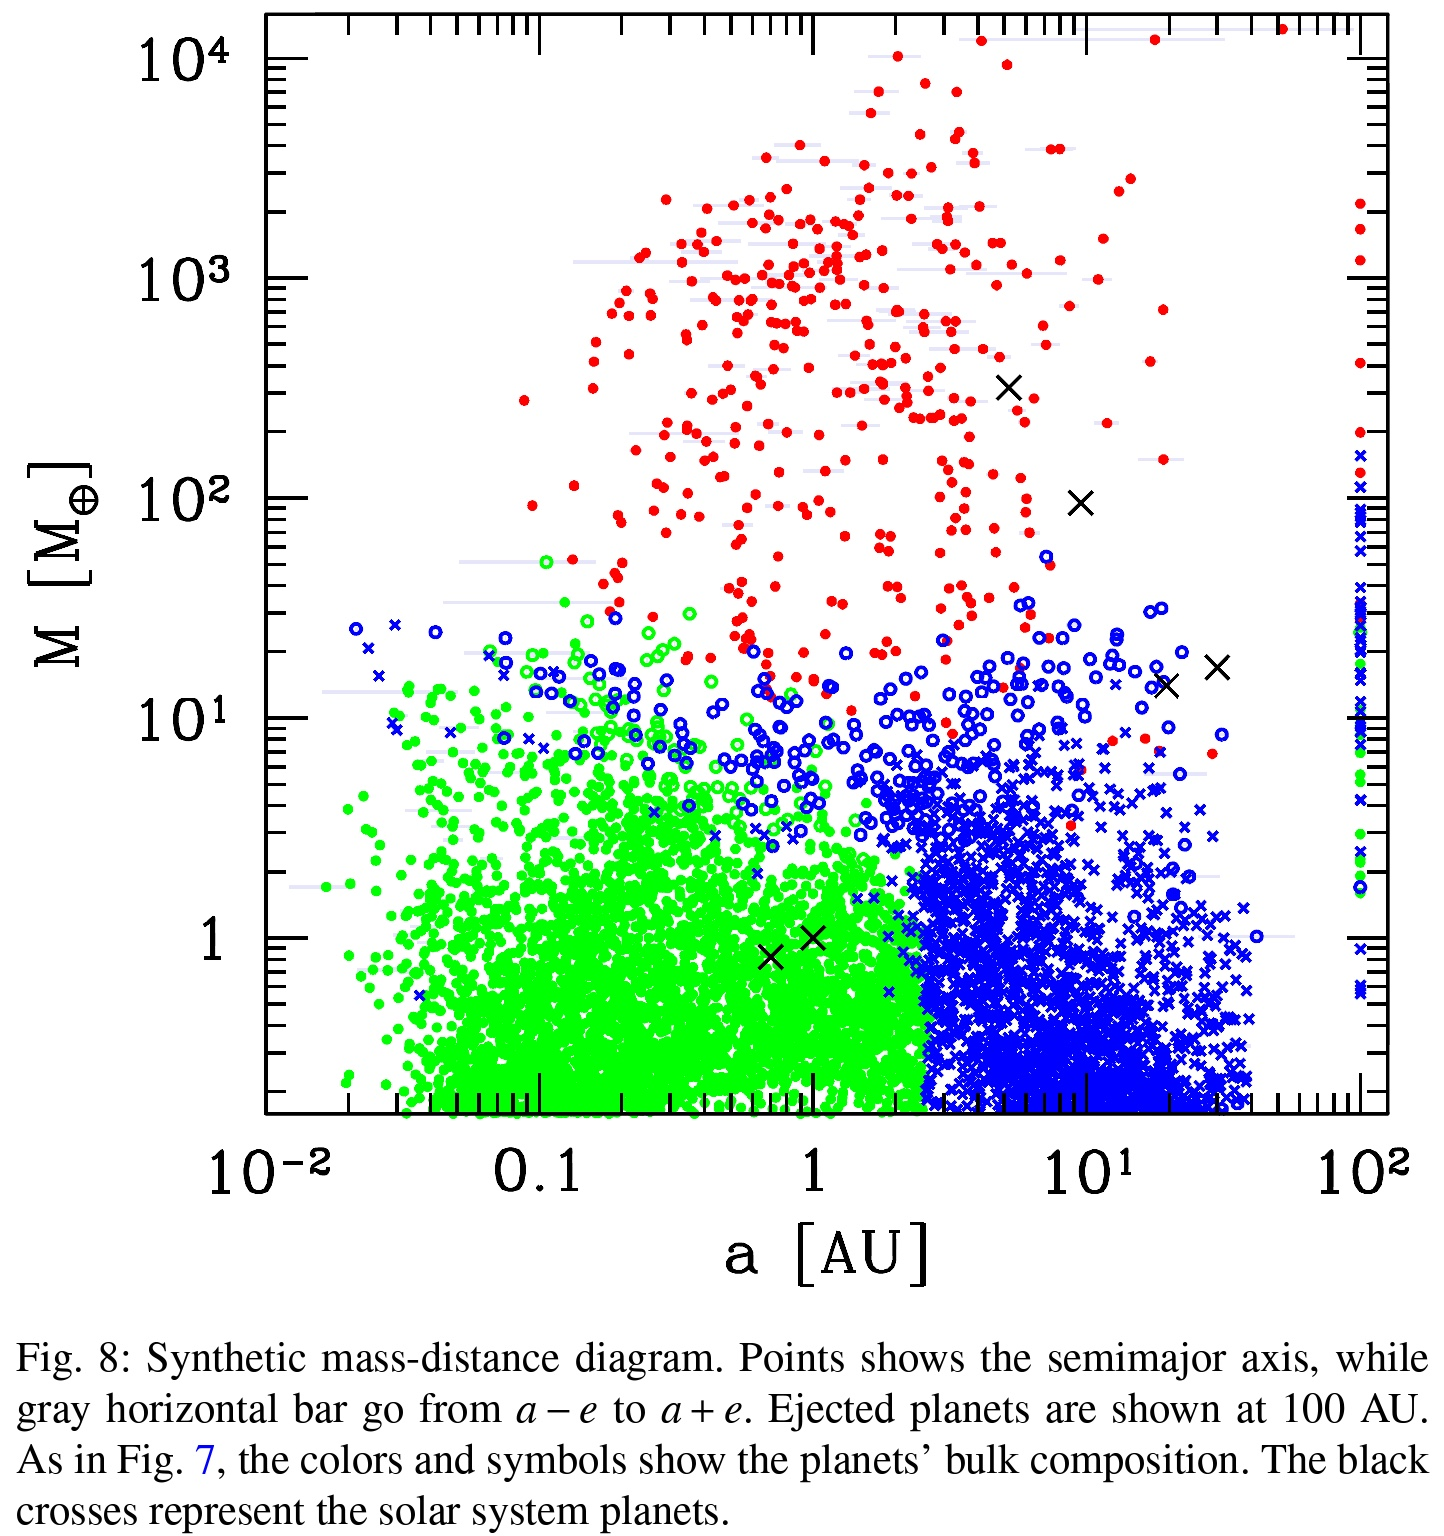
\includegraphics[trim={0cm 8cm 0 0},clip, width=0.8\textwidth,keepaspectratio]{ma-synth}
	\caption{Simulazione popolazione planetaria di 504 sistemi Punti rossi: pianeti giganti con $M_e/M_c>1$; simboli blu/verdi: pianeti che hanno accresciuto core con ghiacci/rocce; punti aperti: $0.1\leq M_{env}/M_{core}\leq1$; croci blu e punti pieni verdi: pianeti con $M_{env}/M_{core}\leq0.1$. Da \cite{mordasini2018planetary}.}\label{fig:ma-synth}
\end{figure}
\end{frame}

\begin{wordonframe}{diagramma M-a}

\end{wordonframe}

\section{Confronto semi-quantitativo simulazione-osservazioni}

\begin{frame}{Confronto pianeti giganti e sistemi compatti}
\begin{table}
	\begin{tabular}{|ccc|}
		\hline
		N&Giganti ($M>300\mearth{}$)&vicini ($P\leq100\si{\day}, R\geq\rearth{}$)\\
		\hline
		1&4.8&8.4\\
		2&7.4&12.8\\
		3&5.4&11.4\\
		4&0.4&10.0\\
		$\geq5$&0.0&11.4\\
		$\exv{S}$&18.0&54.0\\
		O&10-20&50-60\\
		\hline
	\end{tabular}
	\caption{Percentuale di stelle con N pianeti del dato tipo nella popolazione sintetica di \cite{mordasini2018planetary} e confronto con osservazioni.}\label{tab:planetfreq}
\end{table}

\begin{figure}[!ht]
	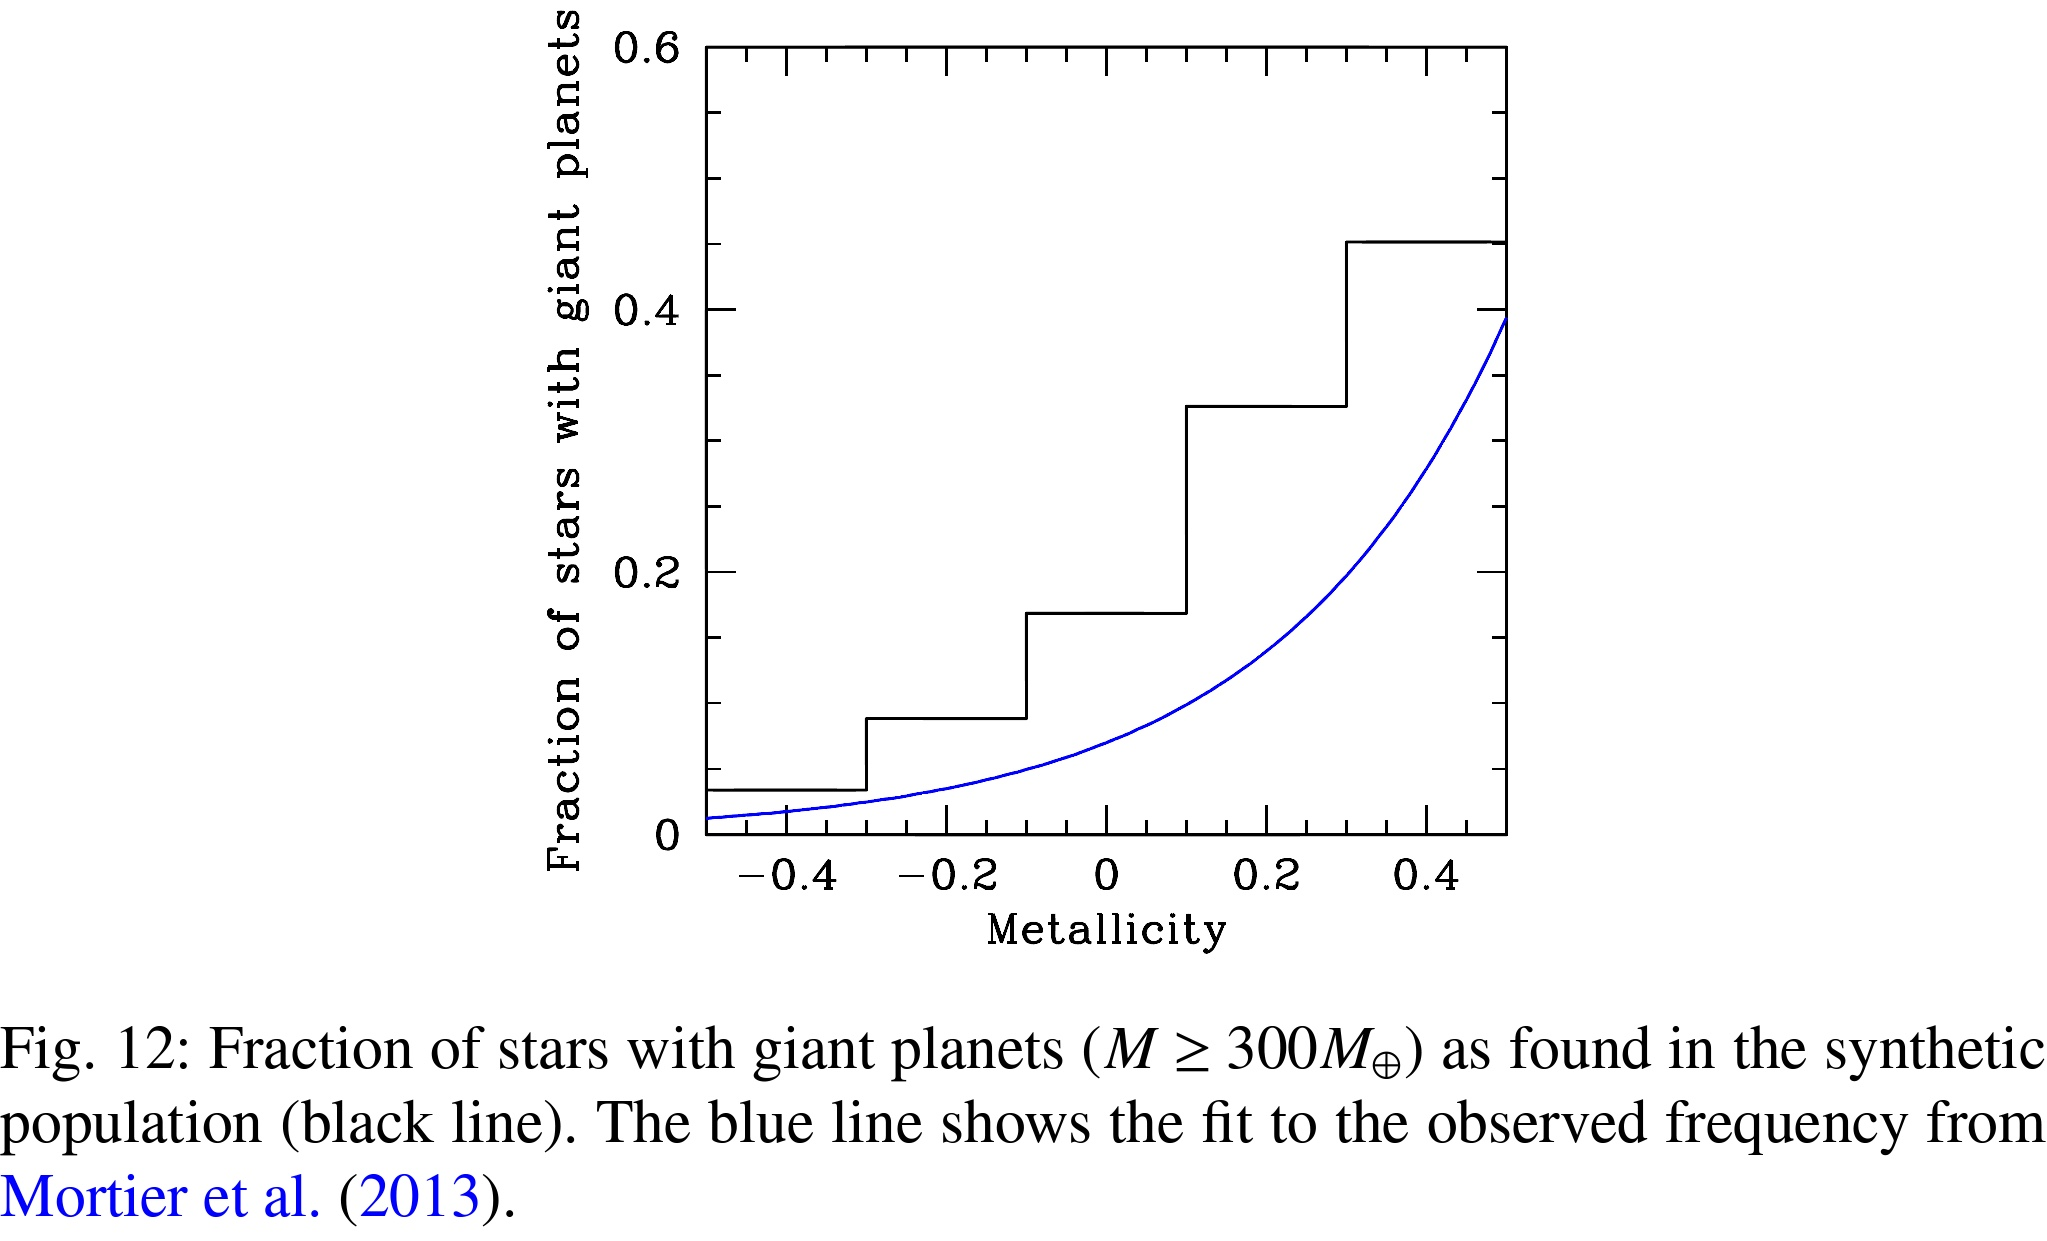
\includegraphics[trim={0cm 10cm 0 0},clip, width=0.9\textwidth,keepaspectratio]{giant-Zsynth}
	\caption{Distribuzione di stelle che ospitano pianeti giganti ($M\geq300\mearth{}$) in funzione della metallicit\'a. Nero: popolazione sintetica. Blu: fit da osservazioni. Da \cite{mordasini2018planetary}. }\label{fig:giant-Zsynth}
\end{figure}
\end{frame}

\begin{wordonframe}{Confronto giganti e compatti -Frequenza vs metallicit\'a}

\end{wordonframe}

\begin{frame}{Confronto pianeti giganti e sistemi compatti}
\begin{figure}[!ht]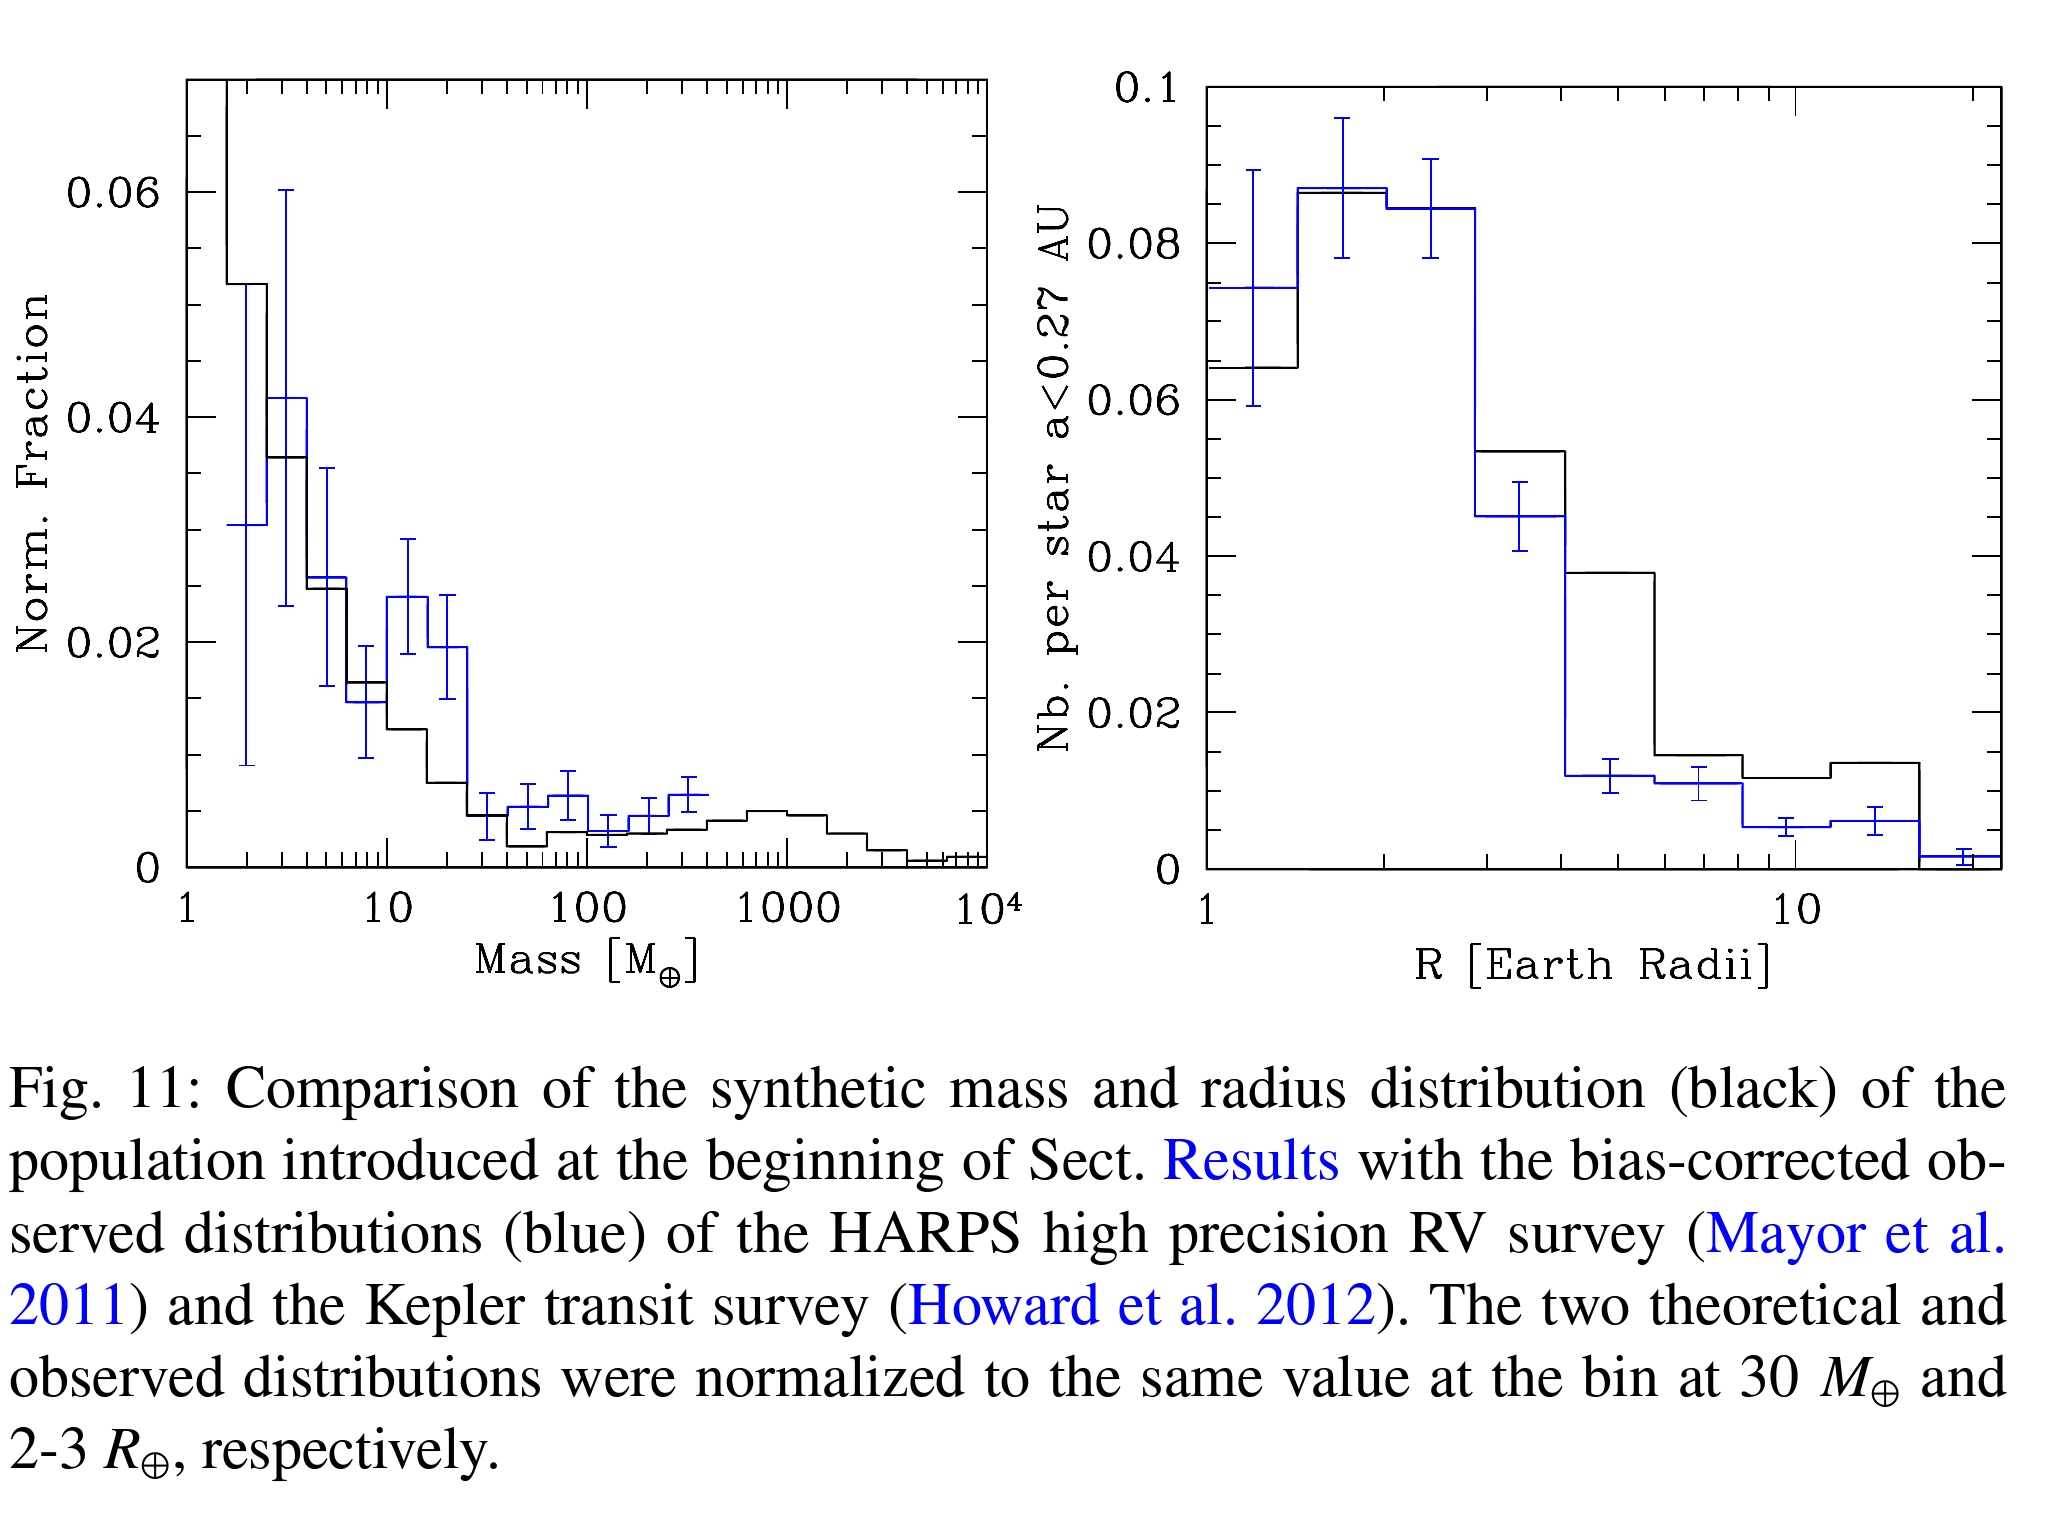
\includegraphics[trim={0cm 17cm 0 0},clip, keepaspectratio,width=0.9\textwidth]{MR-freq-obssynth}\caption{Distribuzioni di massa e raggio per popolazione planetaria sintetica (linea nera) e distribuzioni osservate tramite RV e transiti (linea blu) corrette per i bias. Da \cite{mordasini2018planetary}.}\label{fig:MR-freq-obssynth}\end{figure}
\end{frame}

\begin{wordonframe}{Confronto giganti e compatti -Frequenza vs metallicit\'a}

\end{wordonframe}
